\documentclass{beamer}
\usepackage{pgfpages}
\usepackage[backend=bibtex]{biblatex}
\usepackage{multicol}
\usepackage{multimedia}
\usepackage[absolute,overlay]{textpos}
\usepackage{parskip}
\usepackage{hyperref}
\usepackage{lmodern}
\hypersetup{colorlinks=true, urlcolor=blue}
\setlength{\parskip}{\smallskipamount} 
%\usepackage[texcoord,grid,gridunit=mm,gridcolor=red!10,subgridcolor=green!10]{eso-pic} %DELETE when done with grid
\setbeameroption{hide notes} % Only slides
%\setbeameroption{show only notes} % Only notes
%\setbeameroption{show notes on second screen=right} % Both
%\bibliography{../../papers/references.bib}
\setbeamerfont{footnote}{size=\tiny}
%\AtEveryCitekey{\clearfield{title}}

%
% Choose how your presentation looks.
%
% For more themes, color themes and font themes, see:
% http://deic.uab.es/~iblanes/beamer_gallery/index_by_theme.html
%
\mode<presentation>
{
  \usetheme{Warsaw}      % or try Darmstadt, Madrid, Warsaw, ...
  \usecolortheme{default} % or try albatross, beaver, crane, ...
  \usefonttheme{default}  % or try serif, structurebold, ...
  \setbeamertemplate{navigation symbols}{}
  \setbeamertemplate{caption}[numbered]
} 

\usepackage[english]{babel}
%\usepackage[utf8x]{inputenc} %Doesn't play well with biblatex
\usepackage{amssymb}
\usepackage{bm}
\usepackage{color}
\usepackage{graphicx}

\newcommand{\red}[1]{{\color{red}{#1}}}

\title[{\color{white}{Day 1}}]{{\Huge Sound and Color} \\ {\normalsize Clubes de Ciencia - Ensenada 2017 \\ Frank Wilzcek Course}}
\author{Cody Petrie \& David Rojas}
\institute{Universidad Aut\'onoma de Baja California}
\date{}
\titlegraphic{
\includegraphics[width=2cm]{../../logos/CdeC_logo.png}~%\hspace*{0.75cm}~
   
\includegraphics[width=1.5cm]{../../logos/UABC_logo.png}
}

\begin{document}

%\setbeamertemplate{frametitle}[default][center]
\begin{frame}
   \titlepage
\end{frame}

% Uncomment these lines for an automatically generated outline.
%\begin{frame}{Outline}
%  \tableofcontents
%\end{frame}

% Commands to include a figure:
%\begin{figure}
%\includegraphics[width=\textwidth]{your-figure's-file-name}
%\caption{\label{fig:your-figure}Caption goes here.}
%\end{figure}

\begin{frame}[t]{Synesthesia}
   \begin{itemize}
      \item There is so much in the world that we can't see, smell, hear, taste or touch.
      \item We use technology to enhance our perceptions about the world around us. What are examples?
      \begin{itemize}
         \item<2> Microscopes, \ldots , high energy accelerators
         \item<2> Spyglasses, \ldots , telescopes
         \item<2> Gravitational wave detectors
         \item<2> Radios, \ldots , smart phones
      \end{itemize}
   \end{itemize}
   \only<2>{
   \begin{textblock*}{10cm}(0.3cm,3.7cm) % {block width} (coords)
   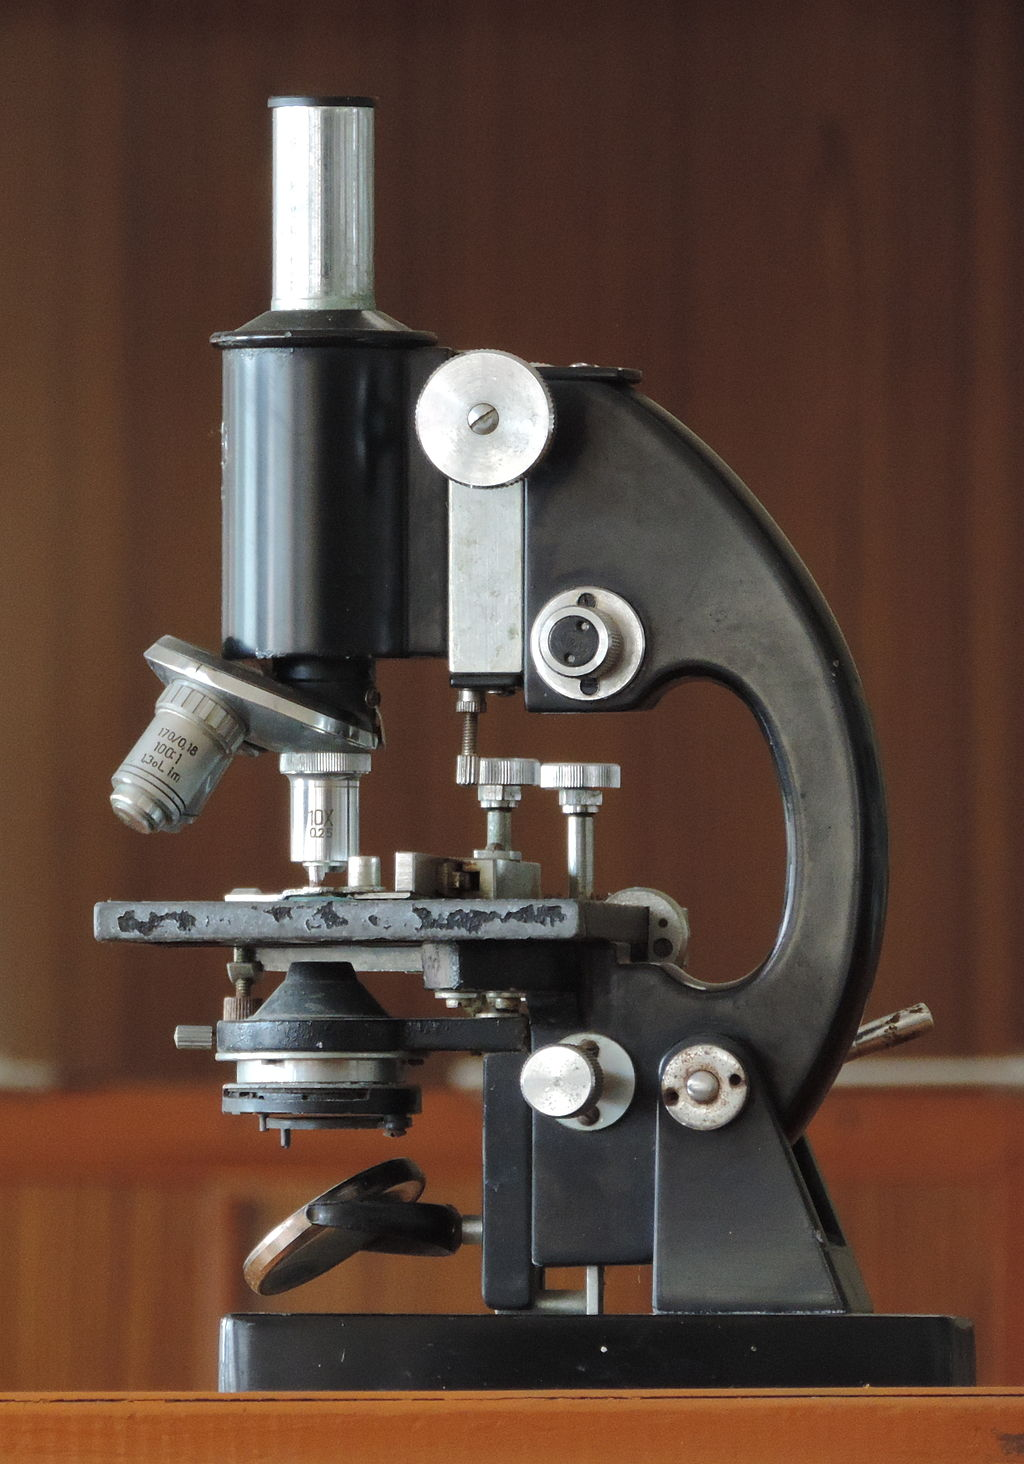
\includegraphics[width=1.7cm]{figures/microscope.jpg}
   \end{textblock*}
   \begin{textblock*}{10cm}(0.3cm,7.2cm) % {block width} (coords)
   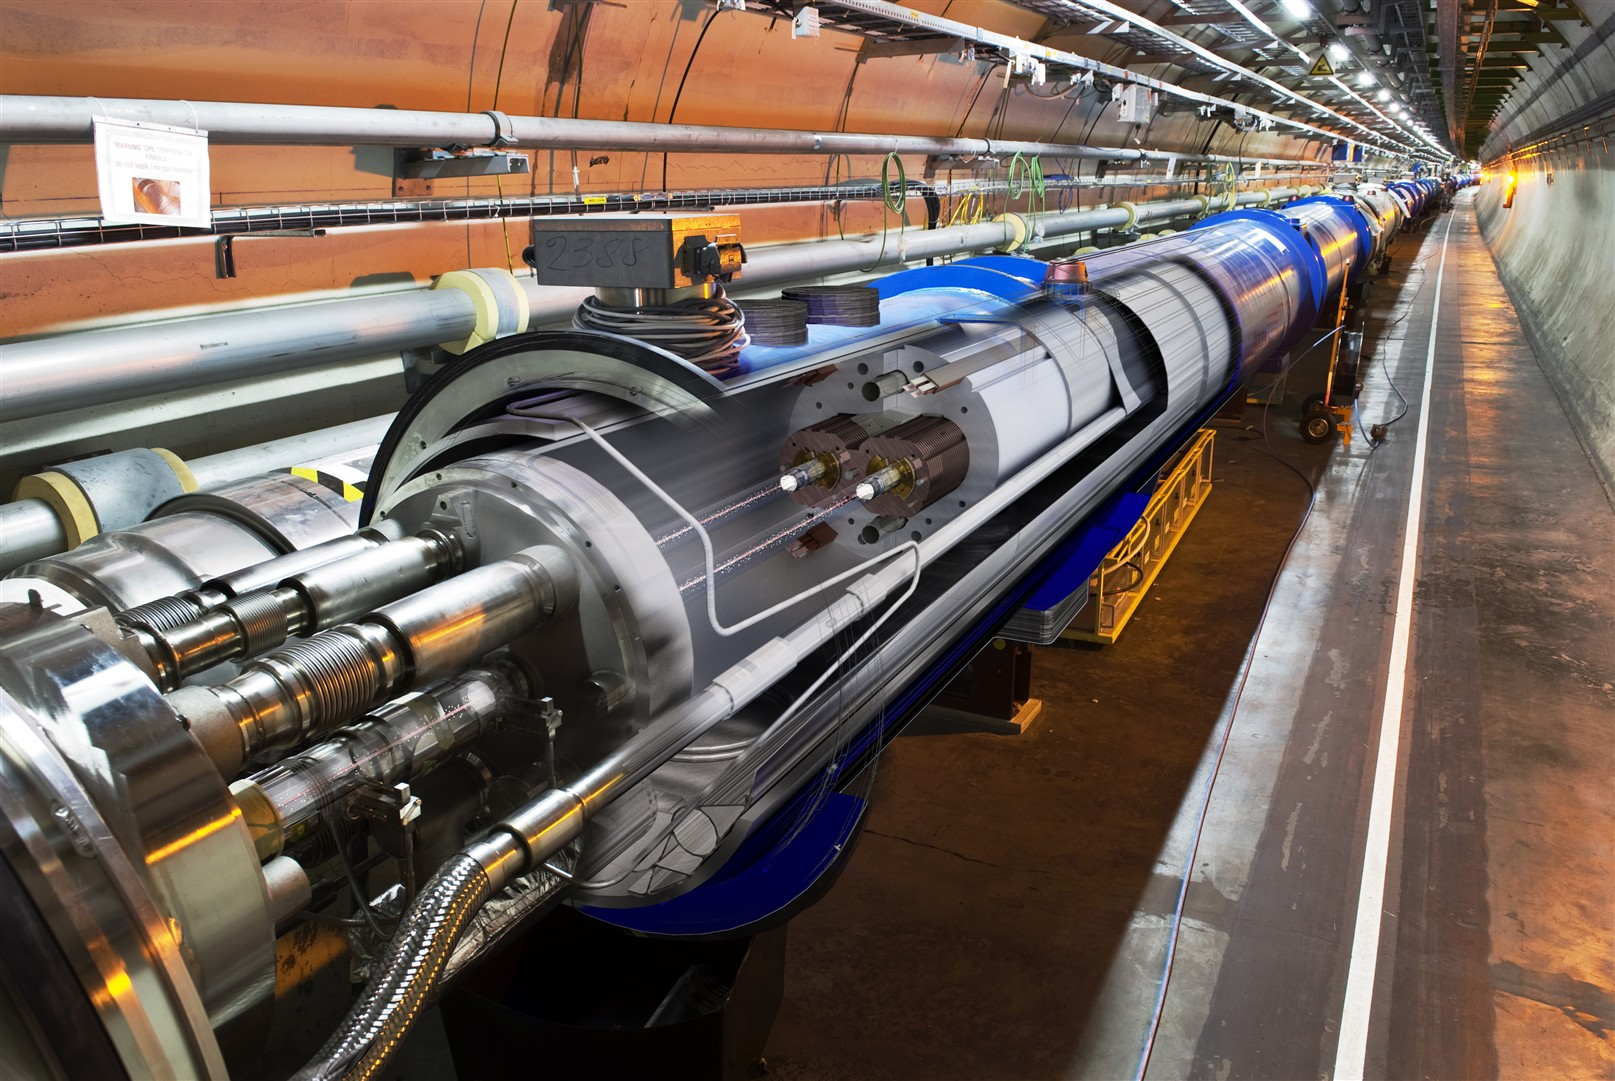
\includegraphics[width=2.7cm]{figures/lhc.jpg}
   \end{textblock*}
   \begin{textblock*}{10cm}(2.9cm,5.4cm) % {block width} (coords)
   
\includegraphics[width=3.2cm]{figures/spyglass.jpg}
   \end{textblock*}
   \begin{textblock*}{10cm}(6cm,7cm) % {block width} (coords)
   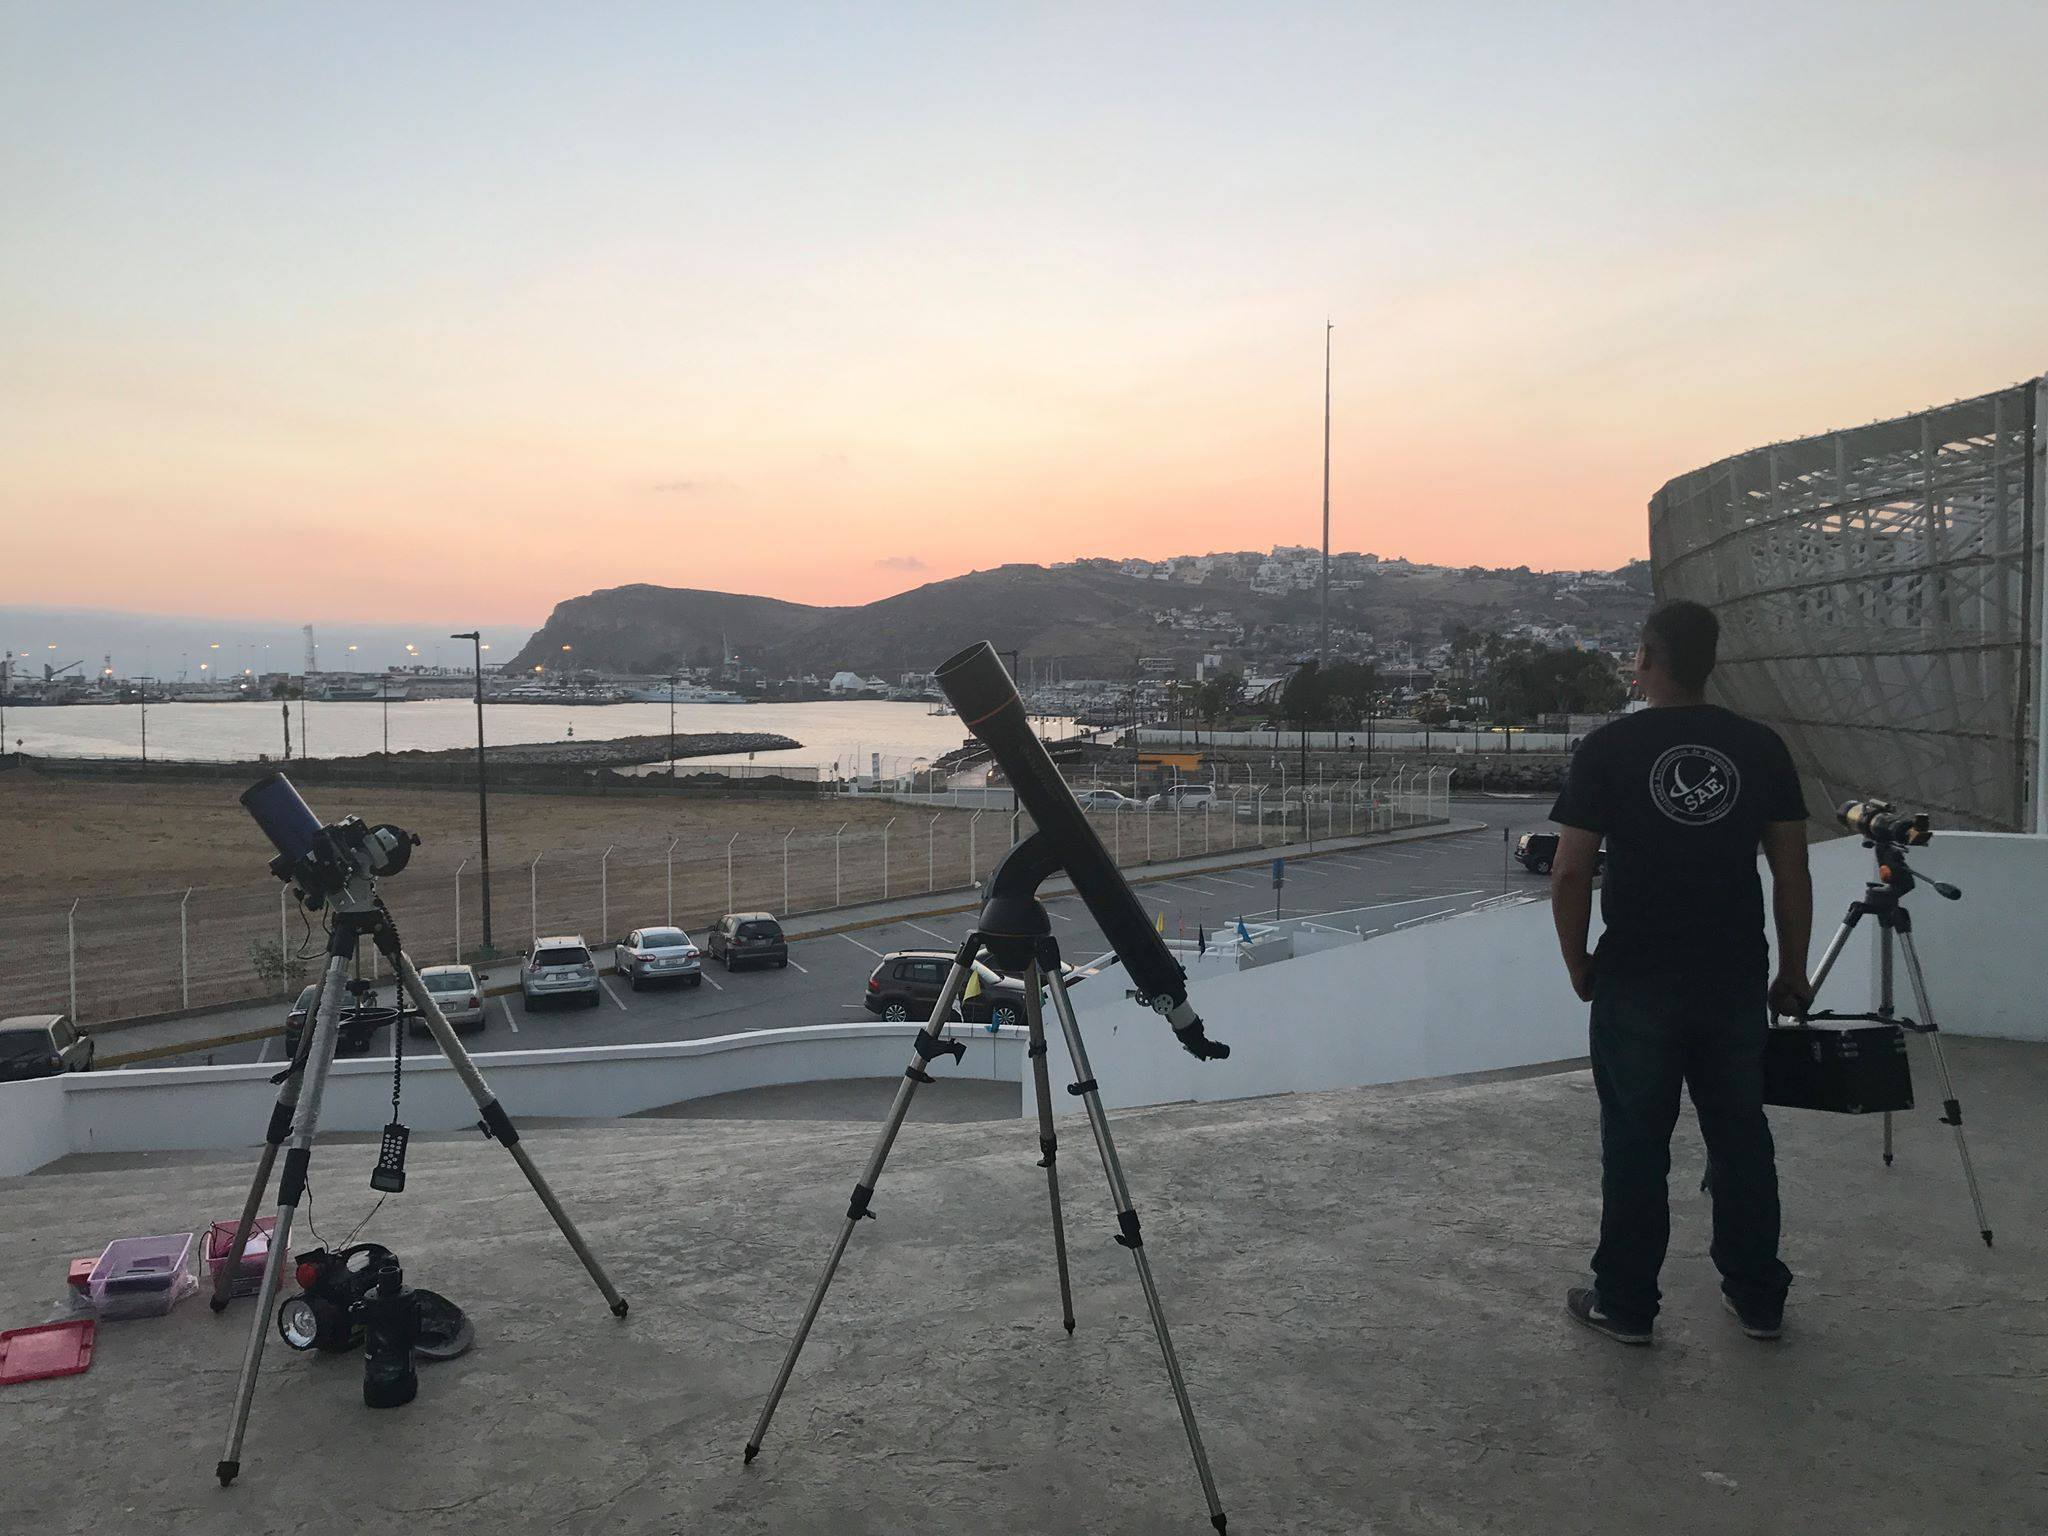
\includegraphics[width=2.9cm]{figures/telescope.jpg}
   \end{textblock*}
   \begin{textblock*}{10cm}(7cm,4.5cm) % {block width} (coords)
   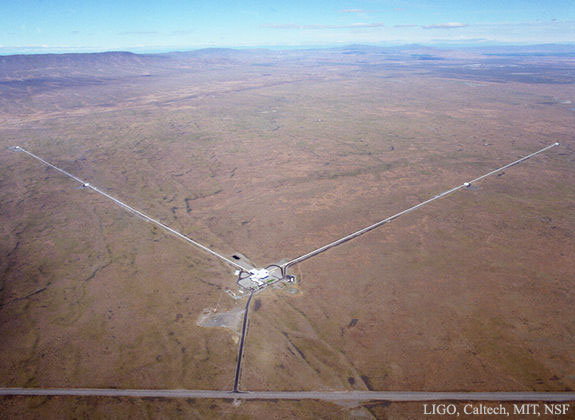
\includegraphics[width=3cm]{figures/gravity.jpg}
   \end{textblock*}
   \begin{textblock*}{10cm}(9.1cm,7.2cm) % {block width} (coords)
   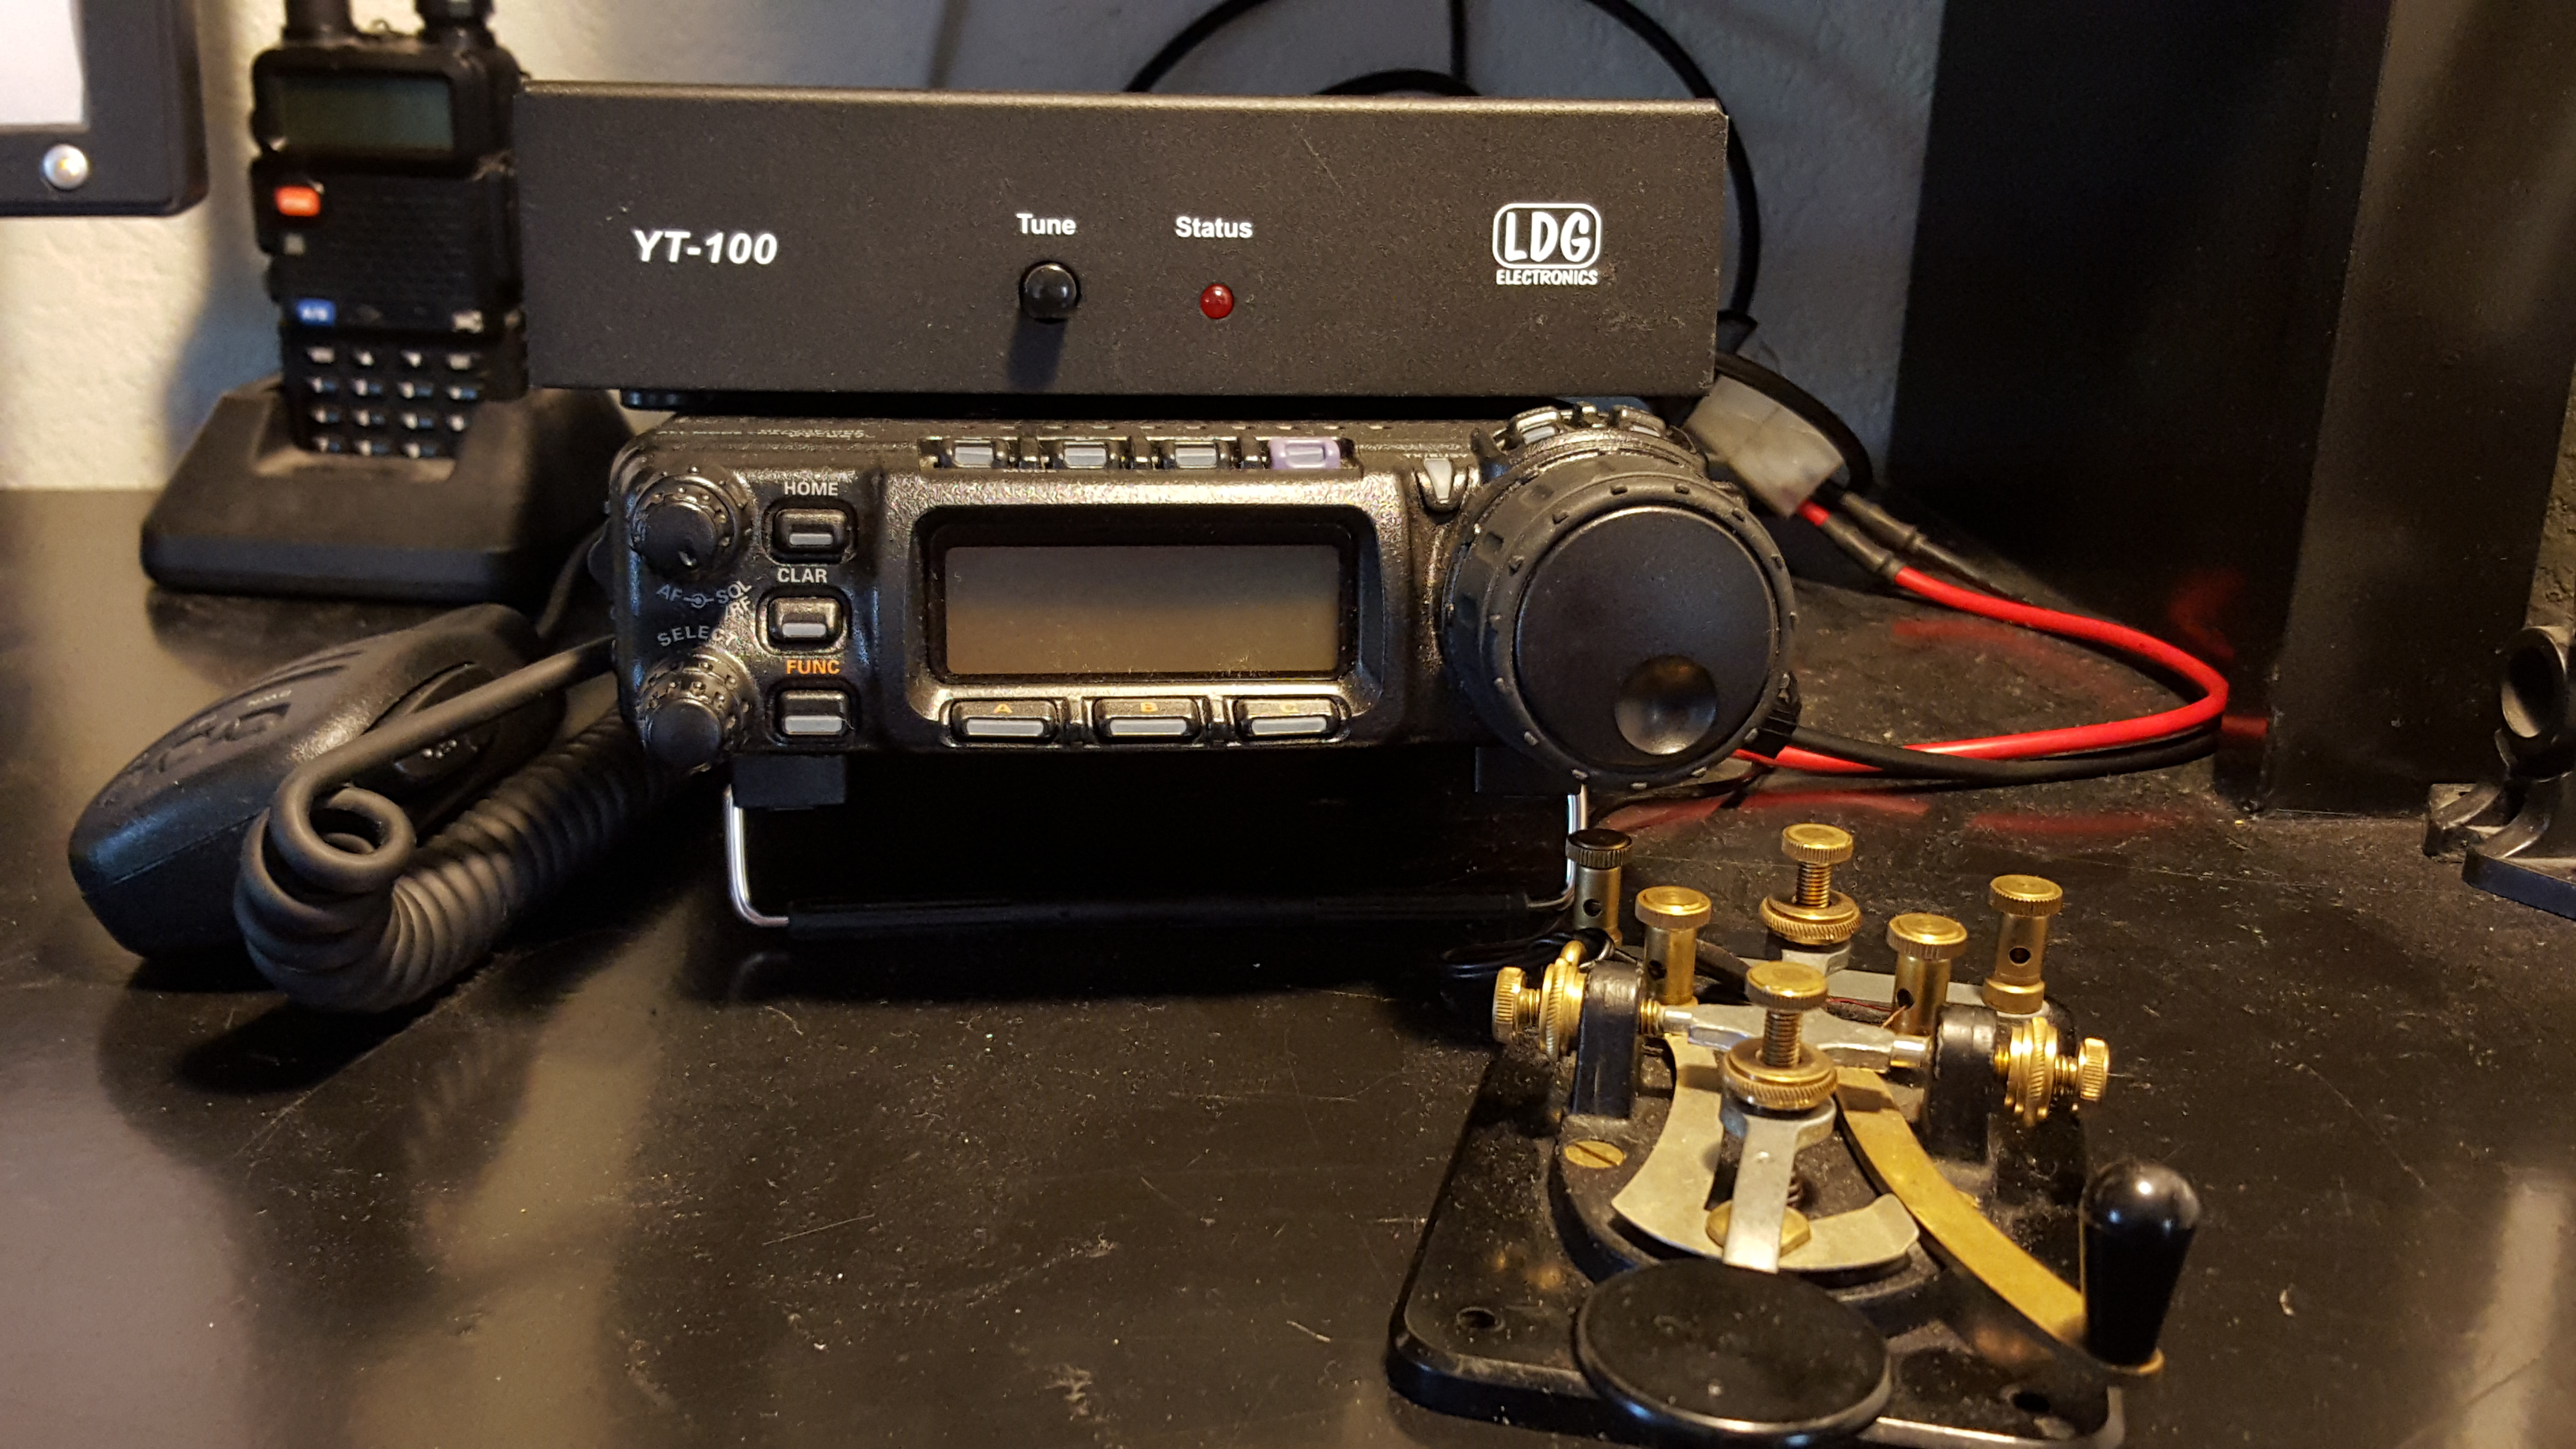
\includegraphics[width=3.5cm]{figures/radio.jpg}
   \end{textblock*}
   \begin{textblock*}{10cm}(10.4cm,3.5cm) % {block width} (coords)
   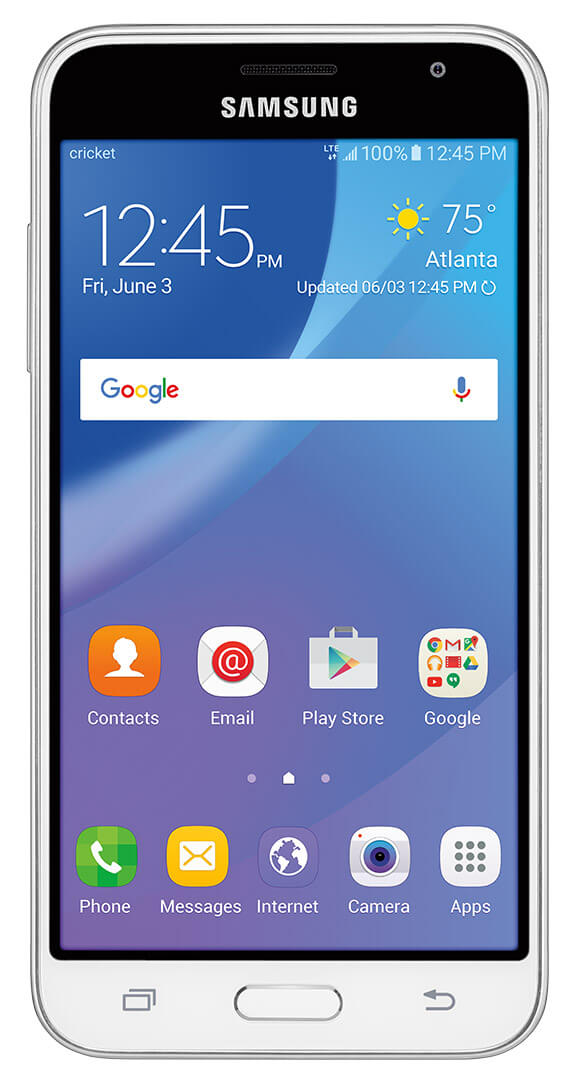
\includegraphics[width=1.7cm]{figures/smartphones.jpg}
   \end{textblock*}
   }
\end{frame}

\begin{frame}{Synesthesia}
   \begin{itemize}
      \item Modern technologies offer us some really exciting opportunities for creative sensory enhancement.
      \item In this course we are going to do this in 4 examples (each of you will participate in 3).
      \begin{enumerate}
         \item Using sound to enhance color vision in software
         \item Using sound to enhance color vision in hardware
         \item Using temporal image processing (TIP) to enhance color vision in software
         \item Using temporal image processing (TIP) to enhance color vision in hardware
      \end{enumerate}
   \end{itemize}
\end{frame}

\begin{frame}{Synesthesia}
   \begin{itemize}
      \item In working these out, you will acquire basic software and hardware skills that you might develop in many directions \\
      \begin{center}
      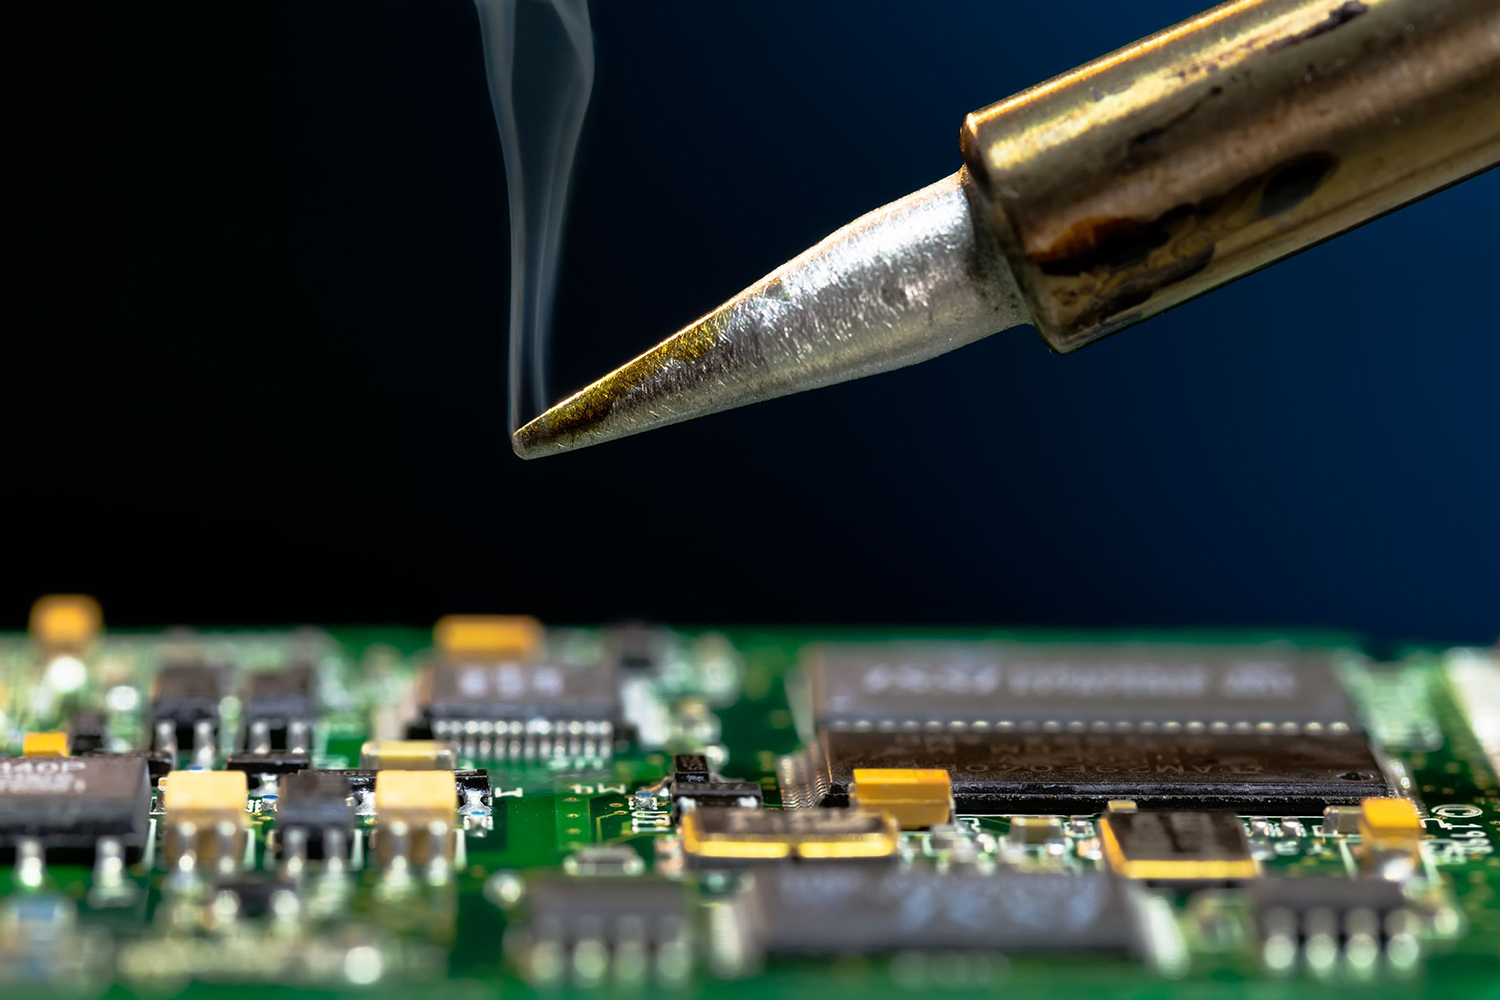
\includegraphics[width=2cm]{figures/solder.jpg}
      ~ ~ ~
      
\includegraphics[width=2cm]{figures/python.png}
      ~ ~ ~
      
\includegraphics[width=2cm]{figures/arduino.png}
      ~ ~ ~
      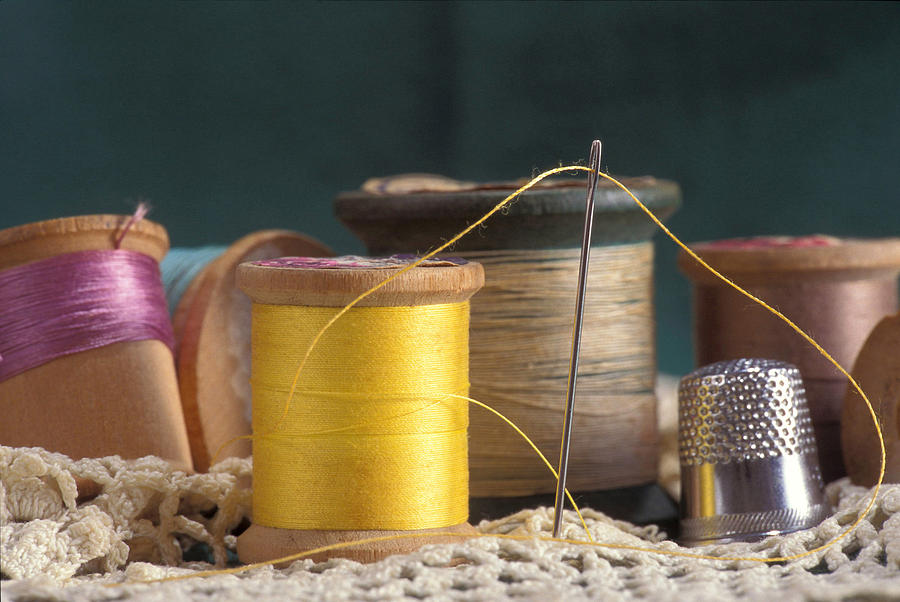
\includegraphics[width=2cm]{figures/sew.jpg}
      \end{center}
      \item We will also discuss general theoretical background, and possibilities for further development of these projects.
      \item We will also introduce you to an exciting new, cutting-edge hyperspectral camera. (We will talk about it, I wansn't able to bring it).
   \end{itemize}
\end{frame}

\begin{frame}{Physics of Light}
   \begin{center}
      \Huge \textcolor{blue}{Physics of Light}
   \end{center}
\end{frame}

\begin{frame}{Physics of Light}
   \begin{itemize}
      \item Visible light is a special case of electromagnetic radiation, which are waves in electric and magnetic fields.
      \begin{center}
         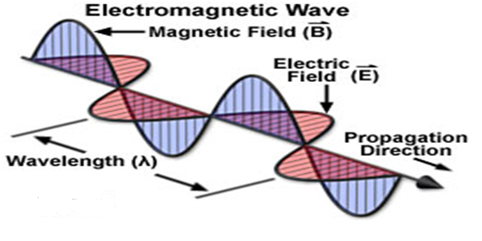
\includegraphics[width=5cm]{figures/emwaves.png}
         ~ ~ ~
         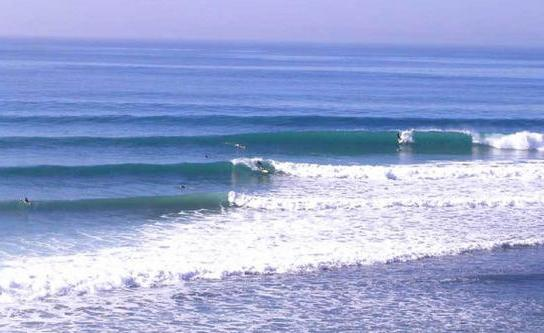
\includegraphics[width=5cm]{figures/oceanwaves.jpg}
      \end{center}
      \item Visible light is simply the part of the infinite spectrum of electromagnetic radiation that our eyes can detect.
   \end{itemize}
\end{frame}

\begin{frame}{Physics of Light}
\begin{center}
   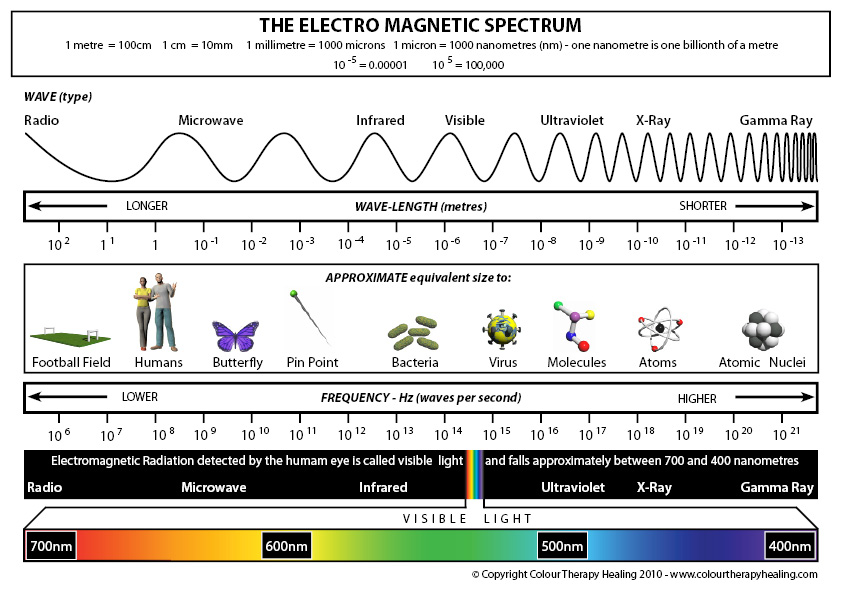
\includegraphics[width=\textwidth]{figures/emspectrum.jpg}
\end{center}
\end{frame}

\begin{frame}{Physics of Light}
\begin{itemize}
   \item Also, the light that we get from the sun mostly comes from the visible part of the spectrum. This is good because that's what we can see, otherwise the world would be a dark place.
   \begin{center}
   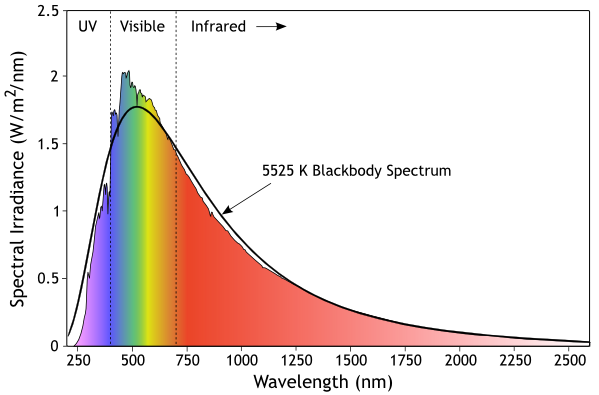
\includegraphics[width=0.9\textwidth]{figures/sunspectrum.png}
   \end{center}
\end{itemize}
\end{frame}

\begin{frame}{Physics of Light}
   \begin{itemize}
      \item Also, the wavelength of visible light is very small on everyday scales. This gives us the ability to resolve small objects with our eyes.
      \begin{center}
      
\includegraphics[width=0.39\textwidth]{figures/me.jpg}
      ~ ~ ~
      
\includegraphics[width=0.38\textwidth]{figures/me_blur.jpeg}
      \end{center}
      \item With visible light we can form sharp images which carry enormously useful information about the sizes and shapes of objects.
   \end{itemize}
\end{frame}

\begin{frame}{Physics of Light}
   \begin{itemize}
      \item This is slightly off topic but sometimes longer wave lengths give us information that we can't see with shorter wave lengths.
      \item This is the cosmic microwave background. Images taken at 21cm to study to radiation left over from the big bang.
      \begin{center}
      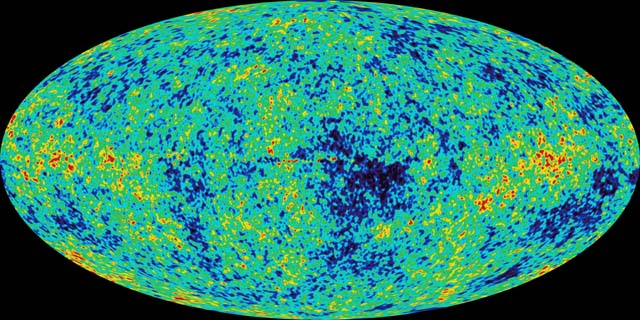
\includegraphics[width=0.8\textwidth]{figures/cmb.jpg}
      \end{center}
   \end{itemize}
\end{frame}

\begin{frame}{Physics of Sound}
   \begin{center}
      \Huge \textcolor{blue}{Physics of Sound}
   \end{center}
\end{frame}

\begin{frame}{Physics of Sound}
   \begin{itemize}
      \item Sound is also a wave, but it's a mechanical pressure/density wave, usually in air, but could be in other media as well.
      \item Unlike visible light which only coveres one octave (430-770 THz) audible sound coveres 10 octaves, or 3 decades.
      \begin{center}
      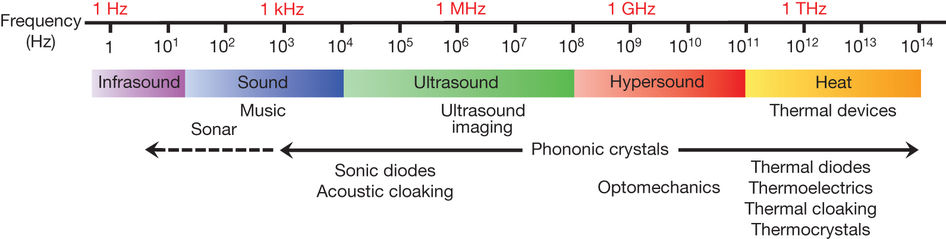
\includegraphics[width=0.8\textwidth]{figures/soundspectrum.jpg}
      \end{center}
   \end{itemize}
   Bumble Bee: 150 Hz \\
   Middle C: 256 Hz \\
   Mosquito: 1500 Hz \\
   Grasshopper: 7 kHz \\
   Bats: 20-200 kHz (Humans top out at $\sim$20 kHz)
\end{frame}

\begin{frame}{Physics of Light}
   \begin{itemize}
      \item The frequencies of audible sounds are closely matched to the sounds of many mechanical objects.
      \begin{itemize}
         \item Vocal cords
         \item Musical instruments
         \item Chair being pushed across the floor
      \end{itemize}
   \end{itemize}
   \begin{center}
      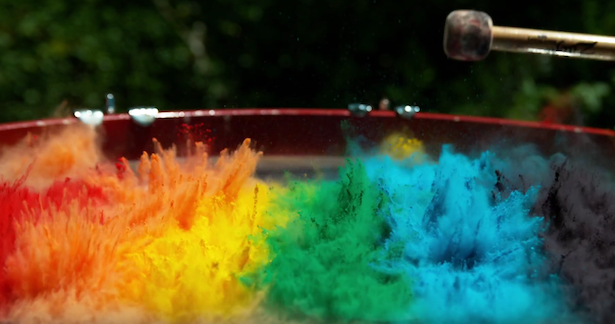
\includegraphics[width=0.8\textwidth]{figures/drum.png}
   \end{center}
\end{frame}

\begin{frame}{Physics of Sound}
   \begin{itemize}
      \item The wavelengths of audible sound are fairly large by the standards of everyday life, as you can infer from the size of musical instruments (and ears).
      \item This makes it difficult to get locate the source of sounds sharply, or to form images.
      \item Bats use {\it ultrasound} and timing of reflected signals to do spatial analysis, as do ultrasound cameras.
   \end{itemize}
   \begin{center}
      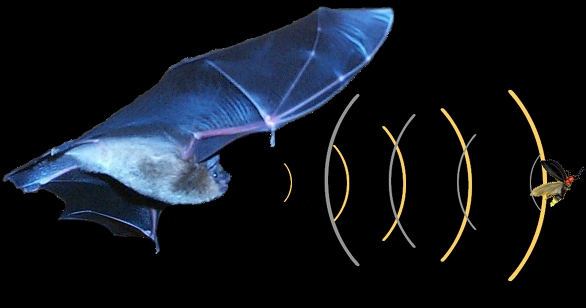
\includegraphics[width=0.5\textwidth]{figures/bat.jpg}
   \end{center}
\end{frame}

\begin{frame}{Physics of Sound}
   \begin{itemize}
      \item Note that ultrasound cameras encode ultrasound information into visual information, so that humans can interpret it readily.
   \end{itemize}
   \begin{center}
      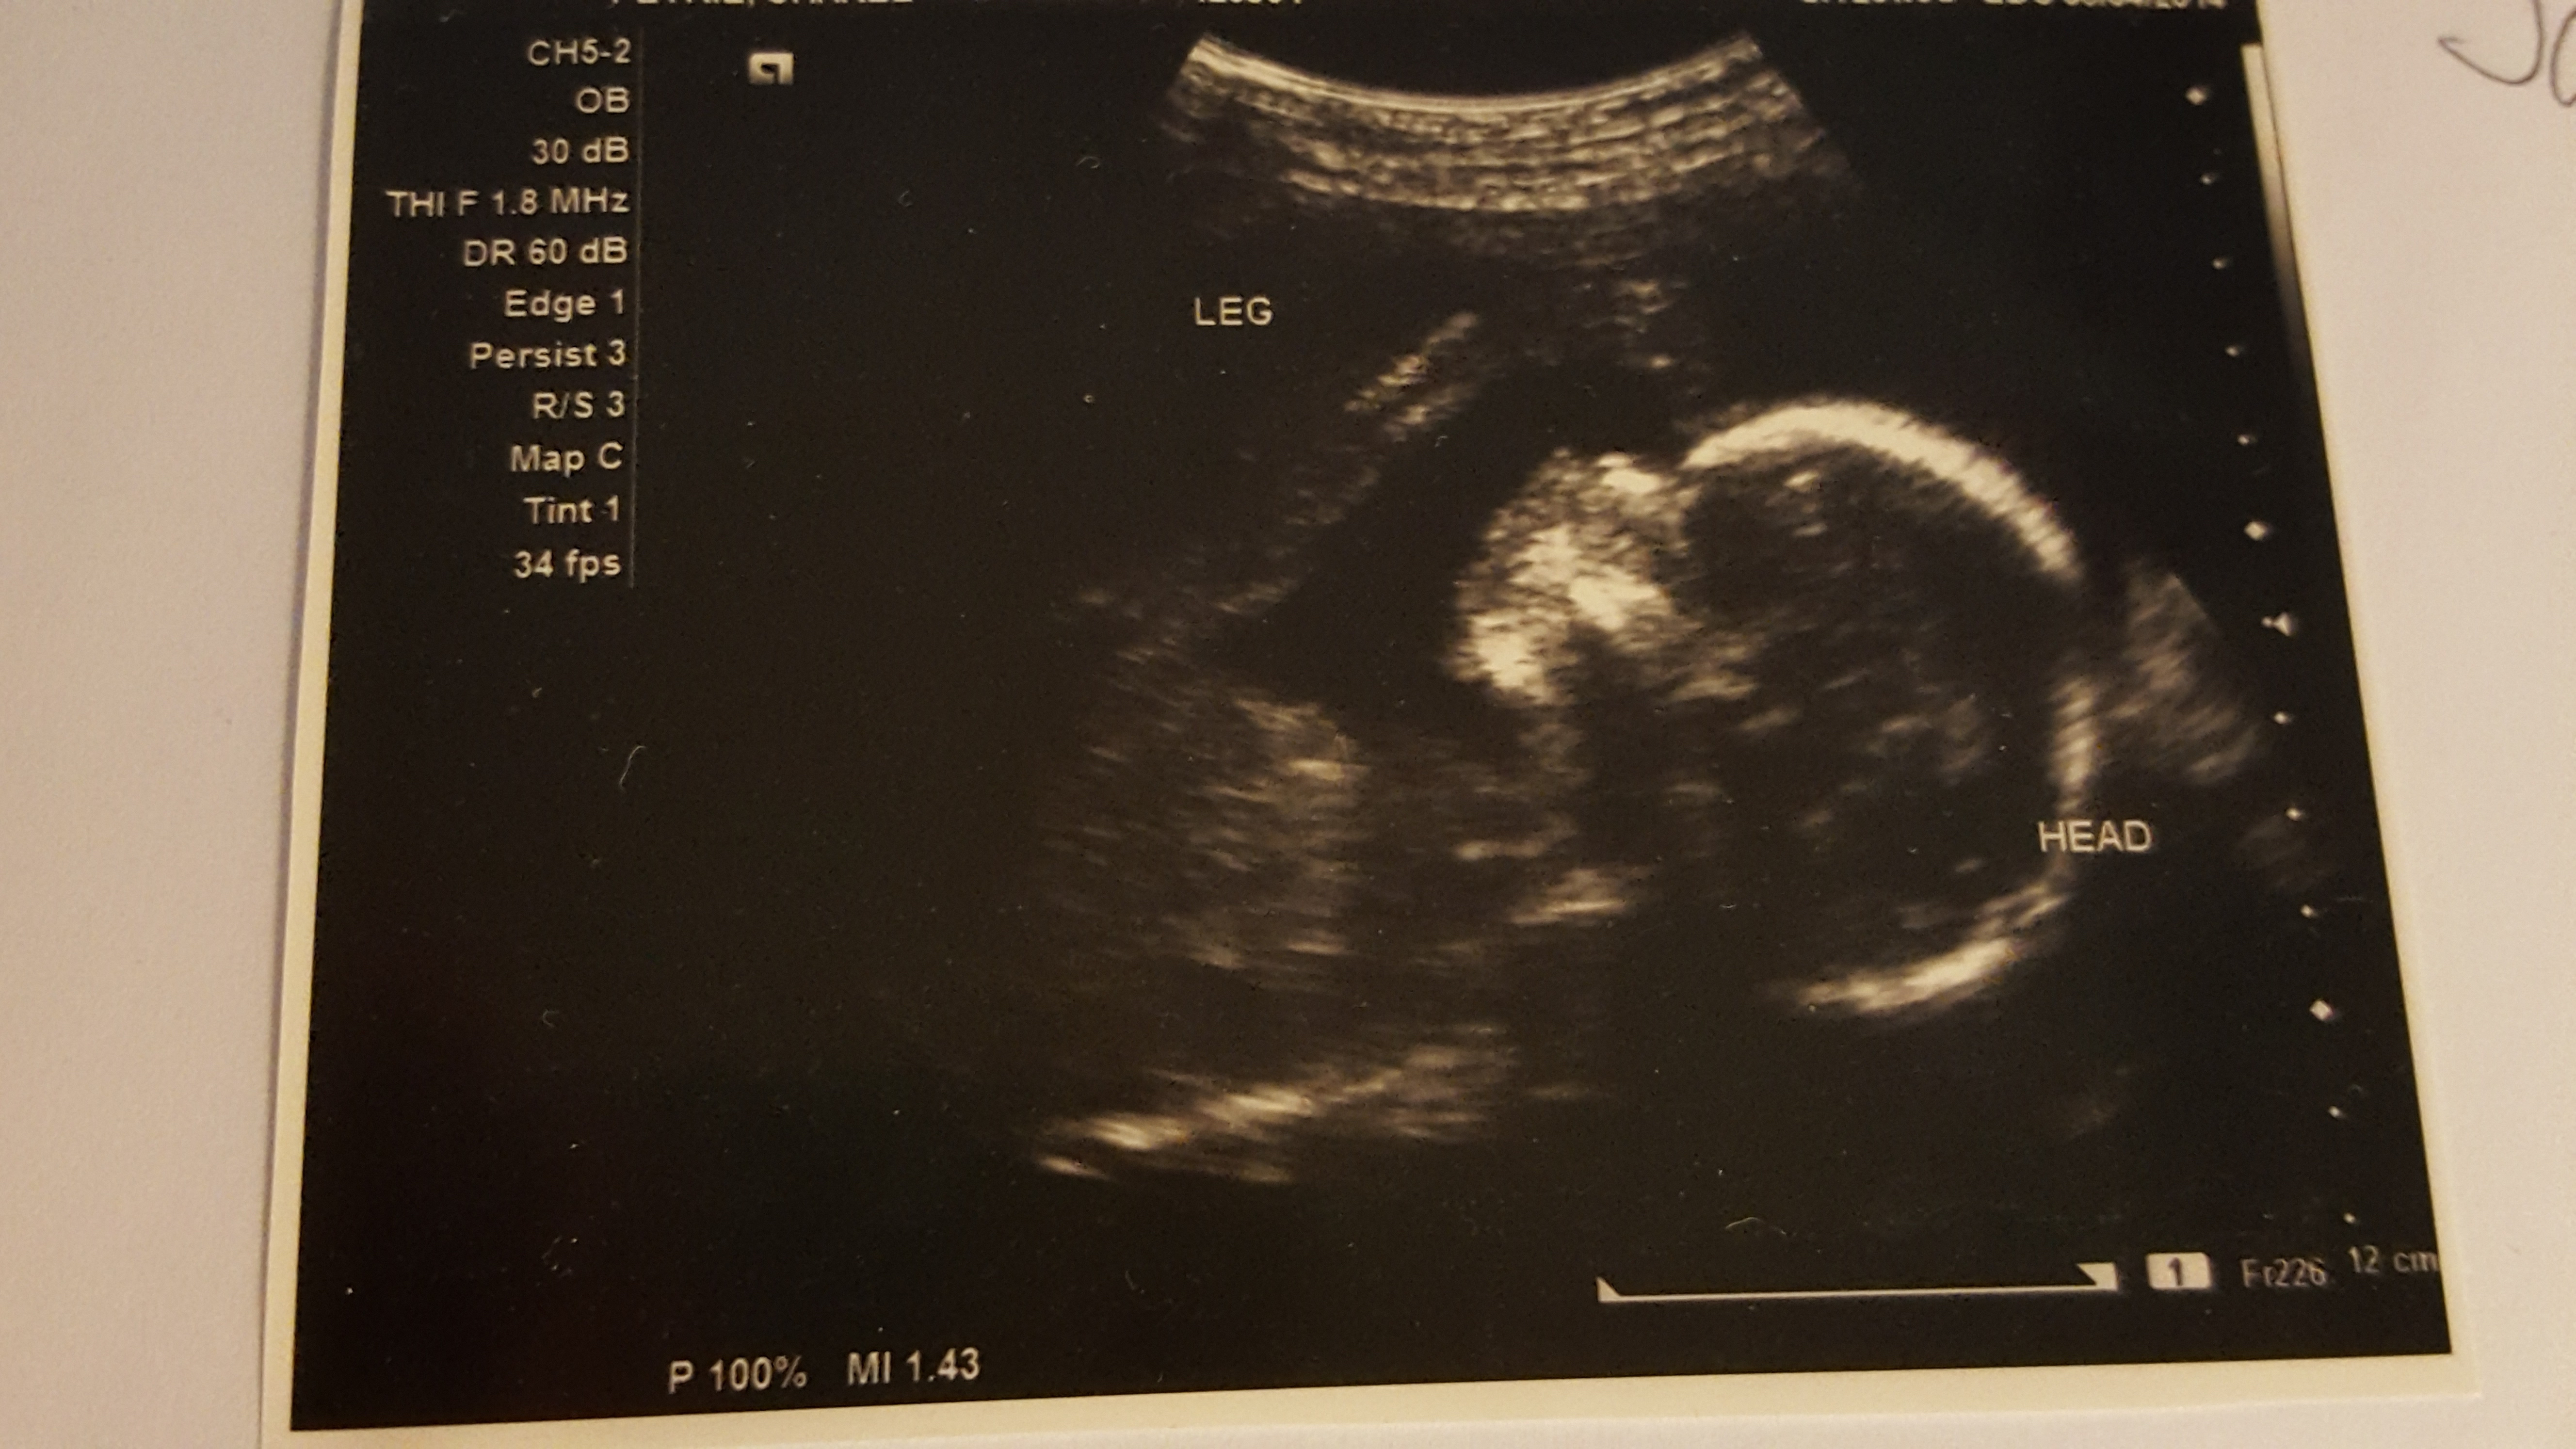
\includegraphics[width=0.9\textwidth]{figures/ultrasound.jpg}
   \end{center}
\end{frame}

\begin{frame}{Light Perception}
   \begin{center}
      \Huge \textcolor{blue}{Light Perception}
   \end{center}
\end{frame}

\begin{frame}{Light Perception}
   \begin{itemize}
      \item Normal human color vision is three-dimensional, or ``trichromatic".
      \item This basic discovery goes back to the nineteenth century. It was made quantitative and precise by James Clerk Maxwell, the same guy who proposed the electromagnetic theory of light.
   \end{itemize}
   \begin{center}
      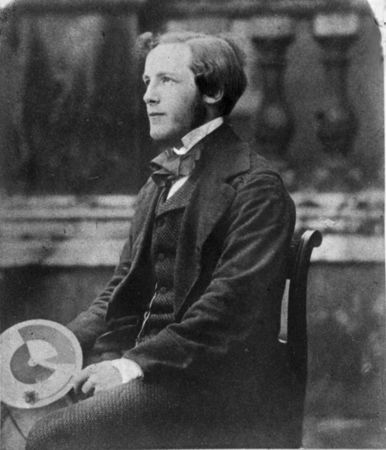
\includegraphics[width=0.4\textwidth]{figures/maxwell.jpg}
   \end{center}
\end{frame}

\begin{frame}{Light Perception}
   \begin{itemize}
      \item His color wheel showed that any color could be perceived by combining the colors red, green and blue in different proportions.
      \begin{center}
         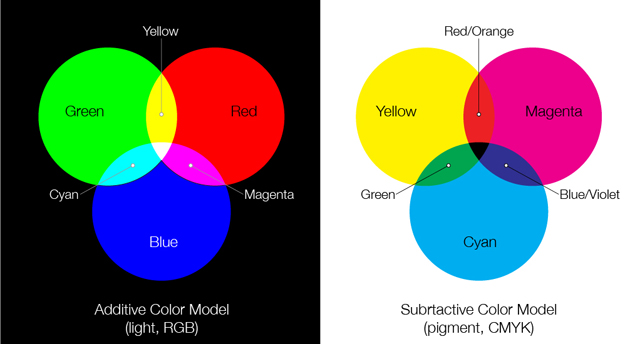
\includegraphics[width=0.9\textwidth]{figures/colors.jpg}
      \end{center}
      \item Note that adding colored pigments is very different from adding colored beams.
   \end{itemize}
\end{frame}

\begin{frame}{Light Perception}
   \begin{itemize}
      \item Human color vision is based on three (RGB) opsins, which are light-sensitive proteins in our retna.
      \item These opsins change shape when they absorb light. These shape changes in the molecules ultimately trigger electrical signals, that is neural impulses. These are the raw input for color vision.
   \end{itemize}
   \begin{center}
      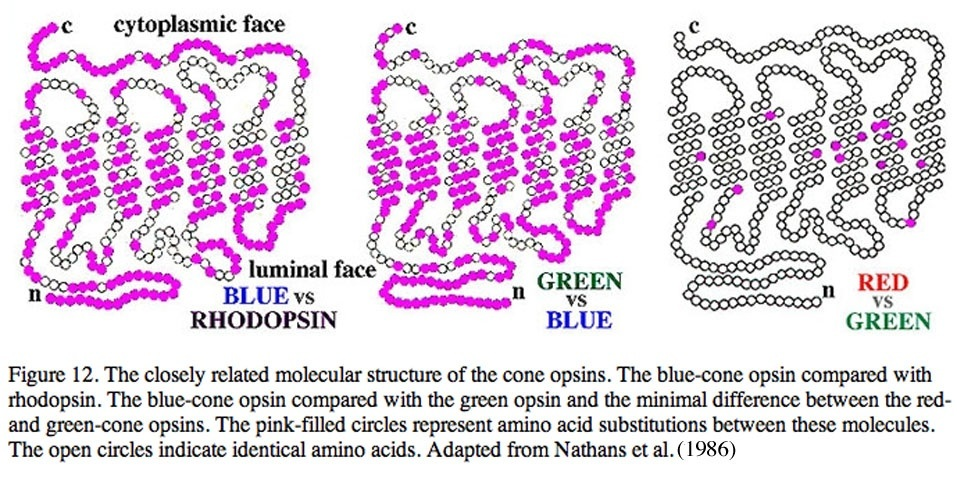
\includegraphics[width=0.8\textwidth]{figures/opsins.jpeg}
   \end{center}
\end{frame}

\begin{frame}{Light Perception}
   \begin{itemize}
      \item These opsin molecules either change shape or they don't, there is no inbetween. Either they absorbed a photon or they didn't and that probability is given by a sensitivity curve - that is, different probabilities for changing shape in response to photons of different frequencies.
   \end{itemize}
   \begin{center}
      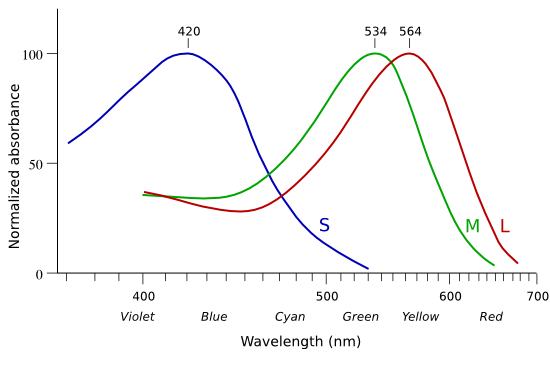
\includegraphics[width=0.9\textwidth]{figures/conecurves.png}
   \end{center}
\end{frame}

\begin{frame}{Light Perception}
   \begin{itemize}
      \item Our brains do a lot of post-processing to turn that raw input - the differential response of three opsins - into color perception!
      \item Many electronic imaging devices do similar post-processing to create images out of combinations of these three colors.
      \item You are going to get some experience doing that yourselves!
   \end{itemize}
\end{frame}

\begin{frame}{Sound Perception}
   \begin{center}
      \Huge \textcolor{blue}{Sound Perception}
   \end{center}
\end{frame}

\begin{frame}{Sound Perception}
   \begin{itemize}
      \item The central ``idea" of auditory perception is sympathetic vibration of a sounding board - the basilar membrane - that has a range of resonant frequencies.
   \end{itemize}
   \begin{center}
      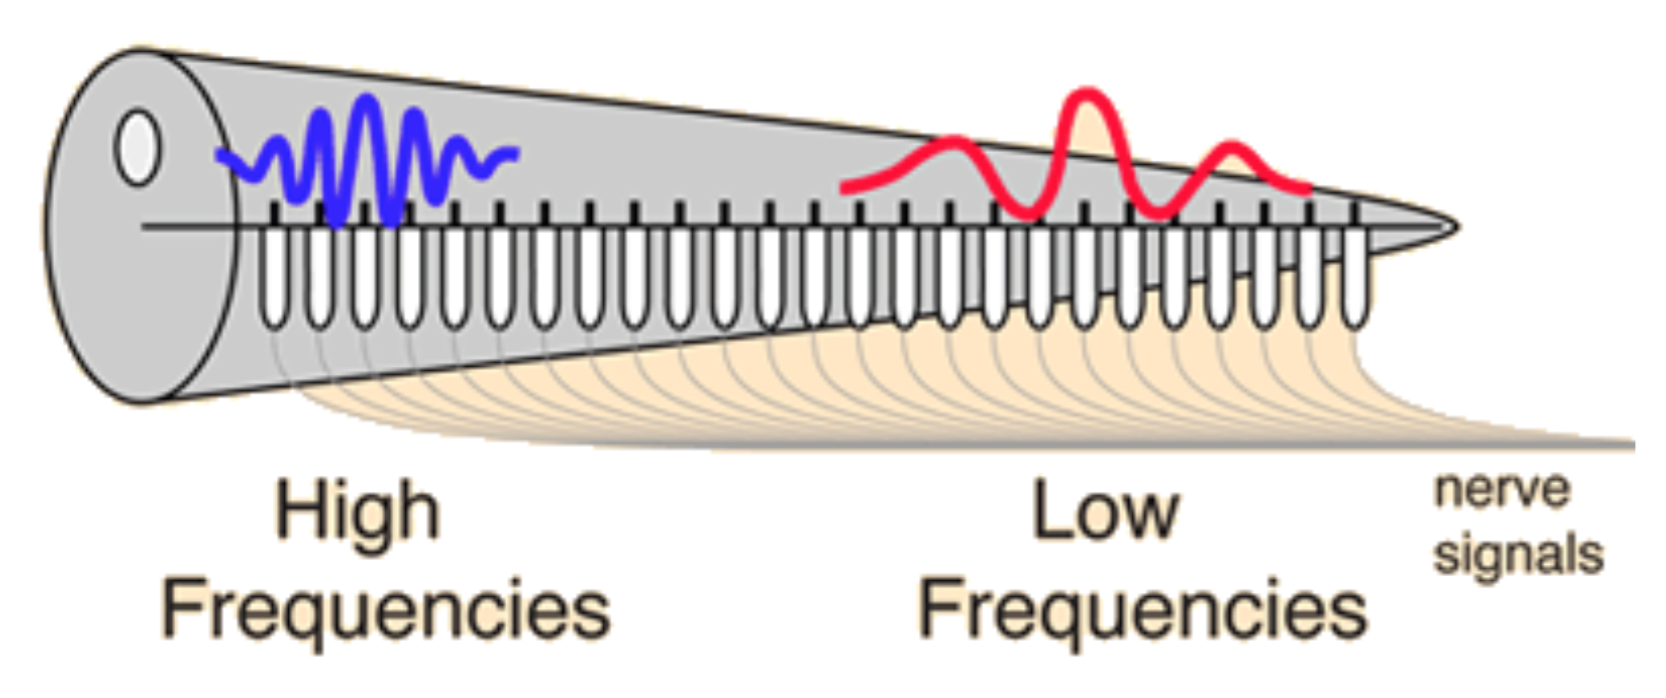
\includegraphics[width=0.9\textwidth]{figures/basilar.png}
   \end{center}
\end{frame}

\begin{frame}{Sound Perception}
   \begin{itemize}
      \item This is like an inverse piano, where the sounds drive the keys.
      \item It performs a spectral (Fourier, you'll see mor on this tomorrow) analysis of the incoming signal.
      \item It does what a prism does for light:
   \end{itemize}
   \begin{center}
      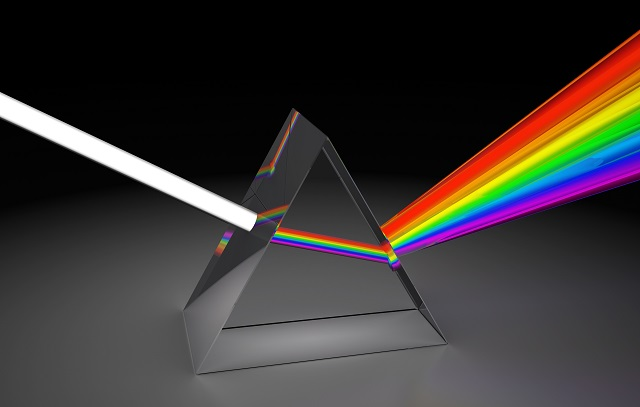
\includegraphics[width=0.8\textwidth]{figures/prism.jpg}
   \end{center}
\end{frame}

\begin{frame}{Sound Perception}
   \begin{itemize}
      \item The complete auditory system has several clever adaptations to impedance match air to fluid, and to keep things reasonably small.
   \end{itemize}
   \begin{center}
      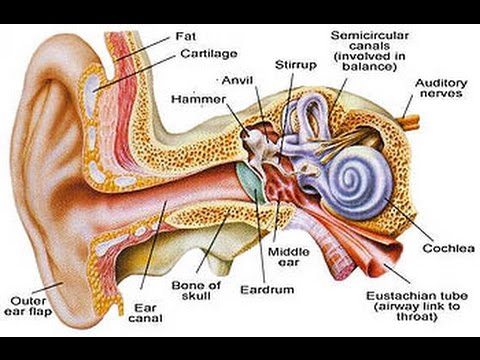
\includegraphics[width=0.8\textwidth]{figures/ear.jpg}
   \end{center}
\end{frame}

\begin{frame}{Comparing Light and Sound Perception}
   \begin{center}
      \Huge \textcolor{blue}{Comparing Light and Sound Perception}
   \end{center}
\end{frame}

\begin{frame}{Comparing Light and Sound Perception}
   \begin{center}
      \begin{tabular}{|c|c|c|}
         \hline
         & & \\
          & Visible Light & Audible Sound \\
         & & \\ \hline
         & & \\
         What is it & Electromagnetic waves & Pressure/density waves \\
         & & \\ \hline
         & & \\
         Wavelength & $\sim$400 - 700 nm & $\sim$17 mm - 17 m  \\
         & & \\ \hline
         & & \\
         Frequency & $\sim$430 - 730 THz & $\sim$20 Hz - 20 kHz  \\
         & (T$\rightarrow 10^{12}$) & \\ \hline
         & & \\
         Energy of Quanta & $\sim$1.5 - 3 eV & Ridiculously small  \\
         & & \\ \hline
      \end{tabular}
   \end{center}
\end{frame}

\begin{frame}{Comparing Light and Sound Perception}
   \begin{center}
      \begin{tabular}{|c|c|c|}
         \hline
         & & \\
         & Visible Light & Audible Sound \\
         & & \\ \hline
         & & \\
         Transceiver strategy & Chemical - & Mechanical - \\
         & bending of molecules & sympathetic vibration \\ \hline
         & & \\
         Quantum important? & Yes & No \\
         & & \\ \hline
         & & \\
         Space analysis & Image formation & Timing and other \\
         & & tricks (crude) \\ \hline
         & & \\
         Time analysis & Color vision (crude) & Harmonic analysis - \\
         & & sounding board \\ \hline
      \end{tabular}
   \end{center}
\end{frame}

\begin{frame}{Hearing More Colors}
   \begin{center}
      \Huge \textcolor{blue}{Hearing More Colors}
   \end{center}
\end{frame}

\begin{frame}{Hearing More Colors}
   \begin{itemize}
      \item Having three cones of colors that we can detect is great, but could be do better?
      \item In principle we could have a rich ``chord" of intensities at each pixel. The mantis shrimp is an inspiration \ldots
   \end{itemize}
   \begin{center}
      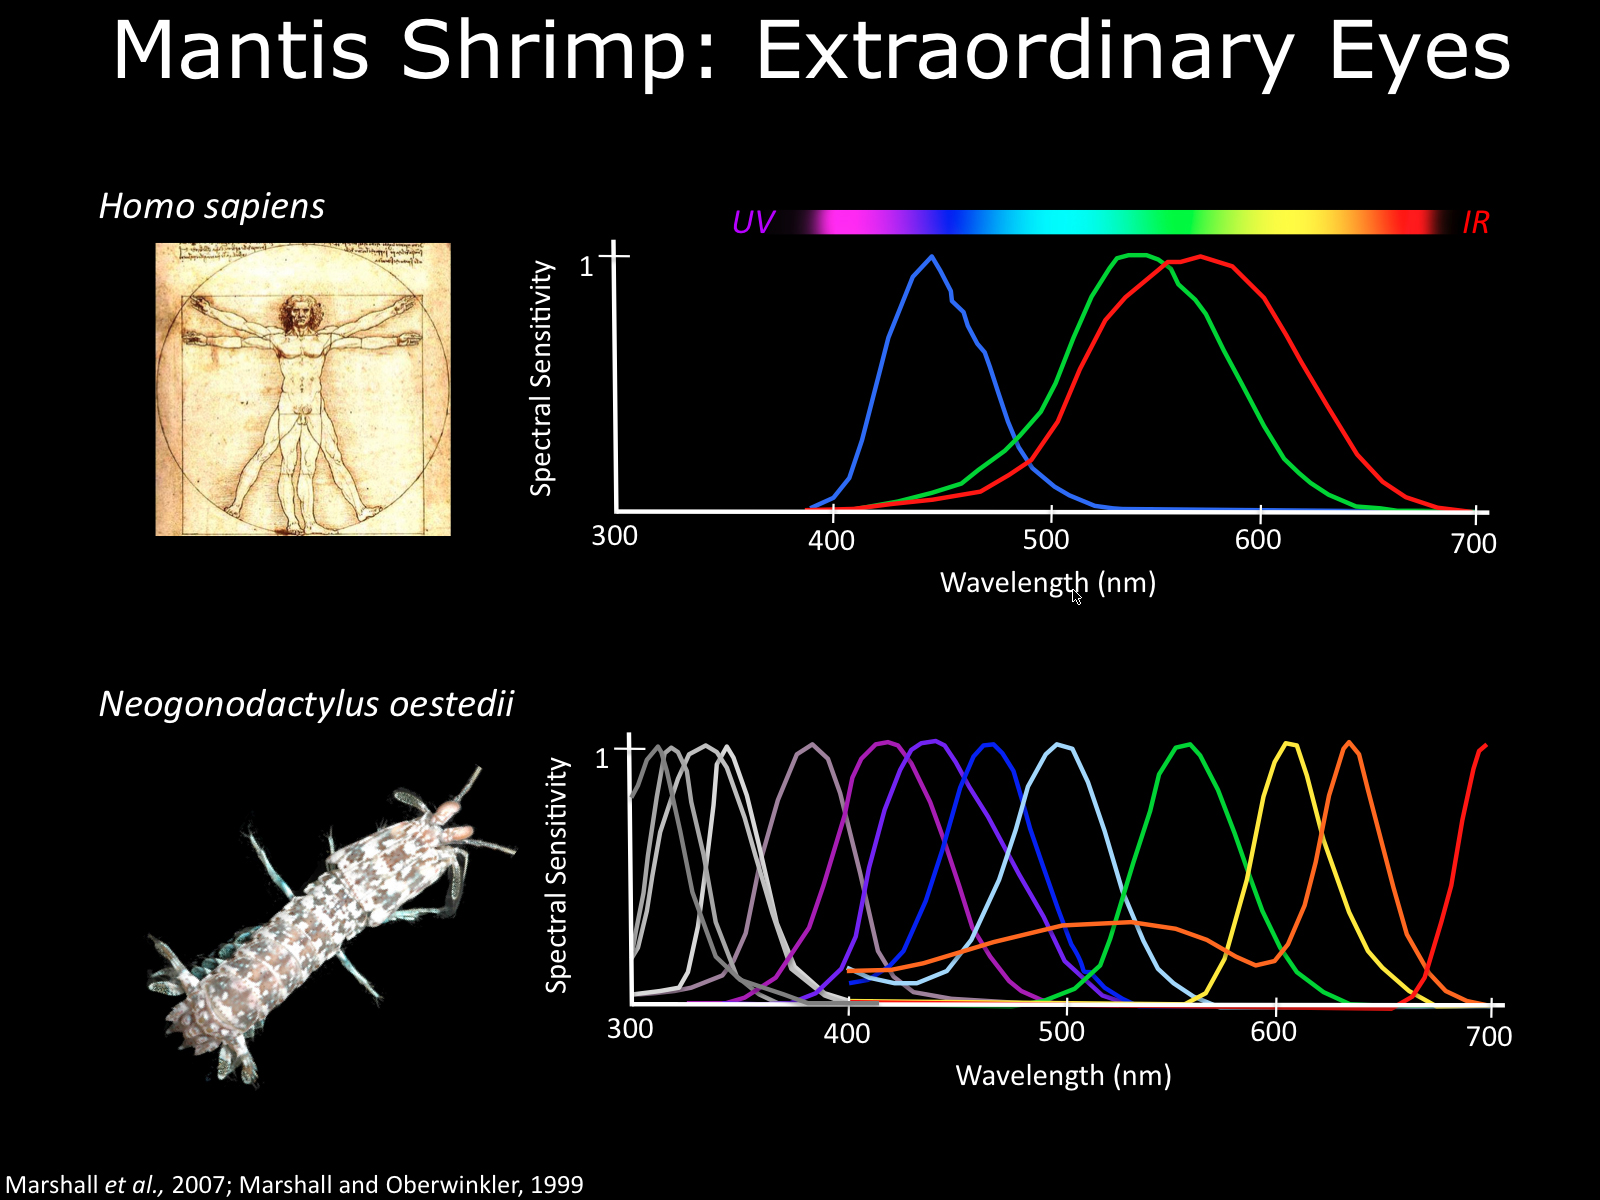
\includegraphics[width=0.7\textwidth]{figures/mantisshrimp.jpg}
   \end{center}
\end{frame}

\begin{frame}{Hearing More Colors}
   \begin{itemize}
      \item Why might this be useful?
      \item Hyperspectral cameras can give us more refined sampling inside and outside the visible spectrum.
      \item We can also have other kind of information associated with images or maps (e.g. temperature, pressure readings, densities of some neurotransmitter or antigen, median income \ldots).
   \end{itemize}
   \begin{center}
      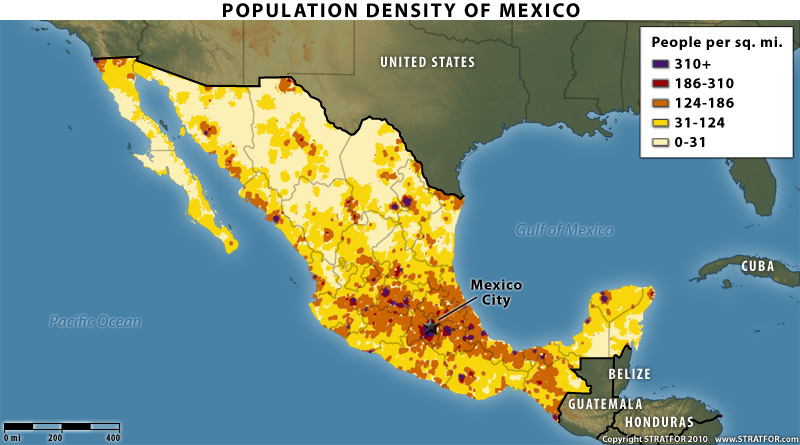
\includegraphics[width=0.7\textwidth]{figures/mexicodensity.jpg}
   \end{center}
\end{frame}

\begin{frame}{Hearing More Colors}
   \begin{itemize}
      \item One way to combine the strengths of vision and audition is to encode multidimensional image files as chords.
      \item That is what we'll be doing, first in software, then in hardware.
   \end{itemize}
\end{frame}

\begin{frame}{Picture Citations}
\fontsize{5}{4}\selectfont 
CdeC logo (accessed 13 July 2017): \href{https://www.clubesdeciencia.mx}{https://www.clubesdeciencia.mx}\\
UABC logo (accessed 13 July 2017): \href{http://www.uabc.mx/}{http://www.uabc.mx/}\\
Microscope (accessed 13 July 2017): \href{https://en.wikipedia.org/wiki/Microscope}{https://en.wikipedia.org/wiki/Microscope}\\
LHC (accessed 13 July 2017): \href{http://www.accelerators-for-society.org/research/index.php?id=5}{http://www.accelerators-for-society.org/research/index.php?id=5}\\
Pirates (accessed 13 July 2017): \href{http://images.yuku.com.s3.amazonaws.com/image/pjpeg/88c16925f7673ba3dc99dffaacc01b48cb41654c.pjpg}{http://images.yuku.com.s3.amazonaws.com/image/pjpeg/88c16925f7673ba3dc99dffaacc01b48cb41654c.pjpg}\\
David with Telescope (accessed 13 July 2017): \href{https://www.facebook.com/profile.php?id=100004290644283\&sk=photos\&collection\_token=100004290644283\%3A2305272732\%3A5}{https://www.facebook.com/profile.php?id=100004290644283\&sk=photos\&collection\_token=100004290644283\%3A2305272732\%3A5}\\
LIGO (accessed 13 July 2017): \href{https://apod.nasa.gov/apod/ap160207.html}{https://apod.nasa.gov/apod/ap160207.html}\\
Smart Phone (accessed 13 July 2017): \href{https://www.cricketwireless.com/cell-phones/smartphones}{https://www.cricketwireless.com/cell-phones/smartphones}\\
Solder (accessed 13 July 2017): \href{https://www.digitaltrends.com/cool-tech/how-to-solder/}{https://www.digitaltrends.com/cool-tech/how-to-solder/}\\
Python logo (accessed 13 July 2017): \href{http://www.bebetterdeveloper.com/coding/hello-world-python.html}{http://www.bebetterdeveloper.com/coding/hello-world-python.html}\\
Arduino logo (accessed 13 July 2017): \href{https://learn.adafruit.com/category/arduino}{https://learn.adafruit.com/category/arduino}\\
Sewing (accessed 13 July 2017): \href{https://fineartamerica.com/featured/needle-and-thread-gerard-fritz.html}{https://fineartamerica.com/featured/needle-and-thread-gerard-fritz.html}\\
EM wave (accessed 13 July 2017): \href{https://www.quora.com/What-is-the-source-of-energy-of-electromagnetic-waves}{https://www.quora.com/What-is-the-source-of-energy-of-electromagnetic-waves}\\
Ocean wave (accessed 13 July 2017): \href{https://wavetribecompany.com/surfing-northern-baja-mexico/}{https://wavetribecompany.com/surfing-northern-baja-mexico/}\\
EM spectrum (accessed 13 July 2017): \href{http://www.colourtherapyhealing.com/colour/electromagnetic-spectrum}{http://www.colourtherapyhealing.com/colour/electromagnetic-spectrum}\\
Sun spectrum (accessed 13 July 2017): \href{https://www.quora.com/Is-the-sun-a-blackbody}{https://www.quora.com/Is-the-sun-a-blackbody}\\
CMB (accessed 13 July 2017): \href{http://cosmology.berkeley.edu/Education/CosmologyEssays/The\_Cosmic\_Microwave\_Background.html}{http://cosmology.berkeley.edu/Education/CosmologyEssays/The\_Cosmic\_Microwave\_Background.html}\\
Sound spectrum (accessed 14 July 2017): \href{https://www.nature.com/nature/journal/v503/n7475/full/nature12608.html}{https://www.nature.com/nature/journal/v503/n7475/full/nature12608.html}\\
Drum (accessed 14 July 2017): \href{http://nerdist.com/a-drum-paint-and-super-slow-mo-is-all-you-need-in-life/}{http://nerdist.com/a-drum-paint-and-super-slow-mo-is-all-you-need-in-life/}\\
Bat (accessed 14 July 2017): \href{http://www.clayton.edu/faculty/sburnett/Bat-Visits/How-do-bats-navigate}{http://www.clayton.edu/faculty/sburnett/Bat-Visits/How-do-bats-navigate}\\
Maxwell (accessed 14 July 2017): \href{https://light2015blog.org/2015/06/12/james-clerk-maxwell-the-man-who-changed-the-world-forever-i/}{https://light2015blog.org/2015/06/12/james-clerk-maxwell-the-man-who-changed-the-world-forever-i/}\\
Opsins (accessed 14 July 2017): \href{https://www.quora.com/What-are-the-chemical-principles-of-the-photoreceptor}{https://www.quora.com/What-are-the-chemical-principles-of-the-photoreceptor}\\
Cone curves (accessed 14 July 2017): \href{http://www.boronine.com/2012/03/26/Color-Spaces-for-Human-Beings/}{http://www.boronine.com/2012/03/26/Color-Spaces-for-Human-Beings/}\\
Prism (accessed 14 July 2017): \href{https://www.azooptics.com/Article.aspx?ArticleID=723}{https://www.azooptics.com/Article.aspx?ArticleID=723}\\
Ear diagram (accessed 14 July 2017): \href{https://i.ytimg.com/vi/01vuuGSd970/hqdefault.jpg}{https://i.ytimg.com/vi/01vuuGSd970/hqdefault.jpg}\\
Mantis shrimp spectrum (accessed 14 July 2017): \href{http://greenforkutah.blogspot.com/2014/07/how-you-can-tell-if-mantis-shrimp-has.html}{http://greenforkutah.blogspot.com/2014/07/how-you-can-tell-if-mantis-shrimp-has.html}\\
Population Density of Mexico (accessed 14 July 2017): \href{https://www.tes.com/lessons/imAOK-WpTHGL1g/comparison-of-mexico-and-venezuela}{https://www.tes.com/lessons/imAOK-WpTHGL1g/comparison-of-mexico-and-venezuela}
\end{frame}

\begin{frame}{Addative (Light) Primary Colors}
   The information for the next two slides comes from \href{http://learn.leighcotnoir.com/artspeak/elements-color/primary-colors/}{http://learn.leighcotnoir.com/artspeak/elements-color/primary-colors/} \\~\\~\\

   Red, green, and blue are the primary colors of light—they can be combined in different proportions to make all other colors. For example, red light and green light added together are seen as yellow light. {\bf This additive color system is used by light sources}, such as televisions and computer monitors, to create a wide range of colors. When different proportions of red, green, and blue light enter your eye, your brain is able to interpret the different combinations as different colors.
\end{frame}

\begin{frame}{Subtractive (Pigment) Primary Colors}
   However, there is another set of primary colors with which you may be more familiar. The primary colors of pigment (also known as subtractive primaries) are used when producing colors from reflected light; for example, when mixing paint or using a color printer. {\bf The primary colors of pigment are magenta, yellow, and cyan (commonly simplified as red, yellow, and blue).}

   {\bf Pigments are chemicals that absorb selective wavelengths}-they prevent certain wavelengths of light from being transmitted or reflected. {\bf Because paints contain pigments, when white light (which is composed of red, green, and blue light) shines on colored paint, only some of the wavelengths of light are reflected.} For example, cyan paint absorbs red light but reflects blue and green light; yellow paint absorbs blue light but reflects red and green light. If cyan paint is mixed with yellow paint, you see green paint because both red and blue light are absorbed and only green light is reflected.
\end{frame}

\end{document}
